%%%%%%%%%%%%%%%%%%%%%%%%%%%%%%%%%%%%%%%%%%%%%%%%%%%%%%%%%%%%%%%%%%%%%%%%%%%%%%%%
%2345678901234567890123456789012345678901234567890123456789012345678901234567890
%        1         2         3         4         5         6         7         8

%\documentclass[letterpaper, 10 pt, conference]{ieeeconf}  % Comment this line out
                                                          % if you need a4paper
\documentclass[a4paper, 10pt, conference]{ieeeconf}      % Use this line for a4
                                                          % paper

\IEEEoverridecommandlockouts                              % This command is only
                                                          % needed if you want to
                                                          % use the \thanks command
\overrideIEEEmargins
% See the \addtolength command later in the file to balance the column lengths
% on the last page of the document

\usepackage[english]{babel}
\usepackage[utf8]{inputenc}
\usepackage[T1]{fontenc}

\usepackage{graphicx} % for pdf, bitmapped graphics files
%\usepackage{epsfig} % for postscript graphics files
%\usepackage{mathptmx} % assumes new font selection scheme installed
%\usepackage{mathptmx} % assumes new font selection scheme installed
\usepackage{hyperref}
\usepackage{booktabs}
\usepackage{multirow}
\usepackage[table,xcdraw]{xcolor}

\title{\LARGE \bf
Unsupervised Machine Learning Algorithms for Edge Novelty Detection
}
\date{April, 2023}

%\author{ \parbox{3 in}{\centering Huibert Kwakernaak*
%         \thanks{*Use the $\backslash$thanks command to put information here}\\
%         Faculty of Electrical Engineering, Mathematics and Computer Science\\
%         University of Twente\\
%         7500 AE Enschede, The Netherlands\\
%         {\tt\small h.kwakernaak@autsubmit.com}}
%         \hspace*{ 0.5 in}
%         \parbox{3 in}{ \centering Pradeep Misra**
%         \thanks{**The footnote marks may be inserted manually}\\
%        Department of Electrical Engineering \\
%         Wright State University\\
%         Dayton, OH 45435, USA\\
%         {\tt\small pmisra@cs.wright.edu}}
%}

\author{\textbf{Candidate:} Ariel Priarone 
\textbf{Supervisor:} Marcello Chiaberge 
\textbf{Co-supervisors:} Umberto Albertin, Gianluca Dara% <-this % stops a space
%\thanks{$^{1}$Department of Electronics and Telecommunications,
%        Politecnico di Torino,
%        Torino, TO, 10129, Italy}%
}

\begin{document}

\maketitle
\thispagestyle{empty}
\pagestyle{empty}

%%%%%%%%%%%%%%%%%%%%%%%%%%%%%%%%%%%%%%%%%%%%%%%%%%%%%%%%%%%%%%%%%%%%%%%%%%%%%%%%
\begin{abstract}
Predictive Maintenance and Novelty Detection are important topics in modern industrial engineering, aimed at proactively identifying equipment failures before they affect system functionality. Embracing these practices is crucial for reducing equipment downtime and optimizing maintenance efforts. Predictive Maintenance aims to quantify and forecast the state of degradation of a system. A quite novel frontier is the direct implementation of Predictive Maintenance within the maintained device, using the principles of Edge Computing.

The fourth industrial revolution is characterized by the integration of Artificial Intelligence and the Internet of Things paradigm into factories. Nowadays, more than a decade since the beginning of this industrial revolution, the maintenance approach remained unchanged in most industrial applications. The primary factor impeding the advancement of the maintenance approach is the significant expense associated with implementing Condition-Based or Predictive maintenance strategies, coupled with a lack of knowledge about the modelling or behaviour of a failing system.

In most facilities, maintenance continues to be performed according to a predefined schedule. An optimization of this approach involves intervening in the system only when necessary, which requires the knowledge of when a system is malfunctioning. Fault Detection and Novelty Detection enable triggering an event when a known fault occurs or when a new, unfamiliar behaviour emerges in the maintained system. 

In this thesis, a framework that performs Novelty Detection is proposed. The structure of the framework is thought to be modular and general-purpose to ease the implementation into different systems. It is developed following an Unsupervised Machine Learning approach to overcome the common lack of physical models of the maintained device. The Machine Learning core of the framework is based on the features extracted from the data gathered from sensors. In the first phase, the data are used to train the models. Then, the framework operates in real time, continuously assessing the status of the system. This solution provides a novelty metric that estimates how unfamiliar the current state of the system is and a forecast of the future evolution of the system.

Firstly, it has been developed to be executed and tested on a PC using various Unsupervised Machine Learning algorithms. The algorithm that appeared to better balance performance and hardware resource consumption was deployed on a microcontroller. The proposed solution includes all the tools necessary in the data pipeline. Relying on the general-purpose structure proposed, the framework can be easily set up on a machine and extended to an arbitrary configuration of sensors and features. 

The PC implementation underwent testing using various Unsupervised algorithms on publicly available datasets, while the edge implementation was tested through laboratory experiments.

Both the tests on datasets and the experimental results showed that the proposed framework is able to detect novelties and give an estimate of the future evolution of the novelty metric of the system.
\end{abstract}

%%%%%%%%%%%%%%%%%%%%%%%%%%%%%%%%%%%%%%%%%%%%%%%%%%%%%%%%%%%%%%%%%%%%%%%%%%%%%%%%
\section{INTRODUCTION}
\label{sec:introduction}

Predictive Maintenance (PM) and Novelty Detection (ND) are important topics in modern industrial engineering, aimed at proactively identifying equipment failures before they affect system functionality. Embracing these practices is crucial for reducing equipment downtime and optimizing maintenance efforts. PM aims to quantify and forecast the state of degradation of a system. A quite novel frontier is the direct implementation of PM algorithms within the maintained device, using the principles of Edge Computing.

\subsection{Motivation}
Despite the Fourth Industrial Revolution, the maintenance approach remained unchanged in many industrial applications. The primary factor impeding the advancement of the maintenance approach is the significant expense associated with implementing PM strategies, coupled with a lack of knowledge about the modelling or behaviour of a failing system.

According to a recent survey by the U.S. Department of Commerce, establishments relying on fixing failures are associated with 3.3 times more downtime than those actively preventing failures. 

\subsection{Objective}
The goal of this project is to design, develop and test a \emph{degradation} based framework
that performs ND using one or several Unsupervised Machine Learning (UML) algorithms. 
The structure of the framework is thought to be modular and general-purpose to ease the implementation into different systems. It is developed following an unsupervised approach to overcome the common lack of physical models and labelled data of the maintained device. This framework has to be deployed for both PC and Edge Computing.
\section{FEATURE EXTRACTION}
The framework is developed to acquire time series data from an arbitrary configuration of sensors. The Field Agent provides time series records according to a predefined cycle or synchronized with the device operation. It ensures that the sampling process is synchronized with the correct sampling frequency. Once a time series is available, the FA extracts the features from the time-domain data. Every time series is linked to a specific set of features to be extracted.

\subsection{Feature set}
The considered features are divided into two categories:
\begin{itemize}
    \item \textbf{Time domain features}: Mean, Standard deviation, Peak-to-peak value (P2P), Root Mean Square value (RMS), Skewness and Kurtosis.
    \item \textbf{Frequency domain features}: Energy of the Wavelet Packet Decomposition (WPD) coefficients, Fast Fourier Transform (FFT) coefficients. The WPD is based on the PyWavelets\footnote{\url{https://github.com/PyWavelets/pywt.git}} library, for Python, and on the Wavelib\footnote{\url{https://github.com/rafat/wavelib.git}} library, for C.
\end{itemize}

The time domain features are computed in the corrected form for sampled data. In the frequency domain, the WPD is preferred in this work, because it reduces the dimensionality of the feature space. The features are standardized along the training dataset, so that the mean and standard deviation are 0 and 1, respectively. This is done to ease the training of the UML algorithms.

\subsection{Scaling and selection}
\begin{figure}
    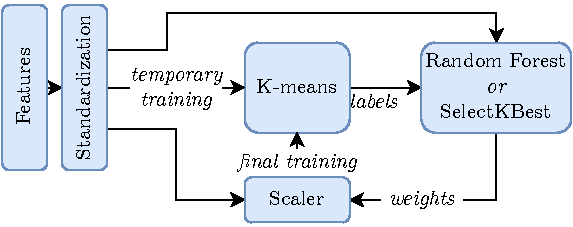
\includegraphics[width=\linewidth]{images/Feat_scaling.pdf}
    \caption{Feature scaling and selection procedure. The features are standardized and then scaled by a weight array or selected to form a smaller feature space. This enhances the performance of the UML models.}
    \label{fig:feature_scaling}
\end{figure}
Despite the standardization, during the experimental validation, it has been observed that some features are more informative than others. To reduce the impact of the less informative features, an optional feature scaling step can be performed. The scaling is done by multiplying the features by a weight array. The weights can be computed by performing a Random Forest training or using the SelectKBest library method. Alternatively, the weights can be used to remove the less informative features, reducing the dimensionality of the feature space. This procedure is shown in Fig.~\ref{fig:feature_scaling}.
\section{PROPOSED FRAMEWORK}
\label{sec:framework}
\begin{figure}
    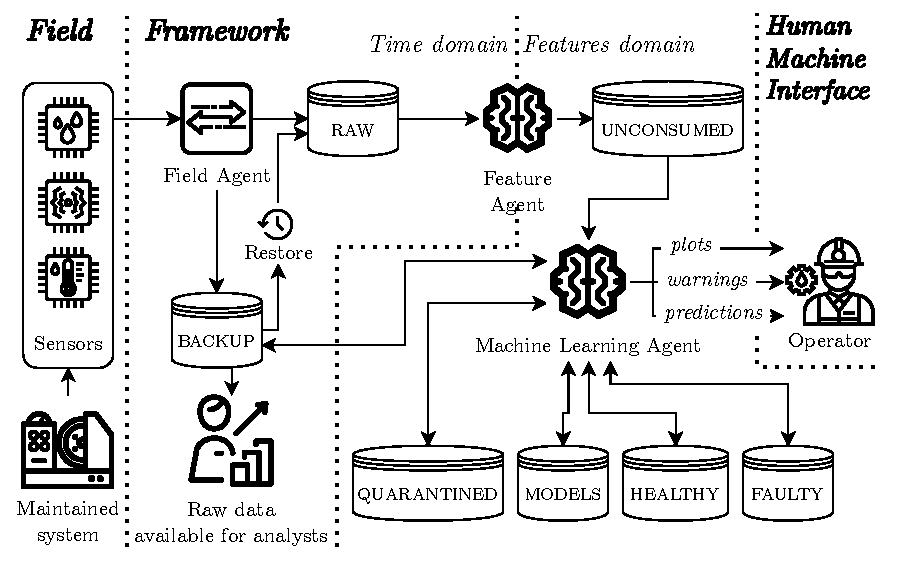
\includegraphics[width=\linewidth]{images/Framework_structure.pdf}
    \caption{The structure of the proposed framework. The Field Agent collects the time series, the Feature Agent extracts the features, and the Machine Learning Agent evaluates the health of the maintained device. The agents are connected to collections of a common database. The 
\includegraphics[height = 1em]{images/DB_icon-cropped.pdf} icon represents a collection of a database that every agent can read and write.}
    \label{fig:framework_structure}
\end{figure}

The solution developed in this thesis is thought to be set up on a new device, and linked to the sensors of the most informative quantities of the system.
In the first phase of commissioning, the framework collects the data, extracts the features and stores them. When the collected data are enough to characterize all the modes of operation of the maintained system, the UML model can be trained. Finally, the framework continues collecting new time series, extracting the features and evaluating these new samples. Now, the framework produces a Novelty Metric (NM) that quantifies how anomalous the new data are. 
This phase lasts indefinitely (until the maintenance team performs a model update). When the NM overshoots a certain threshold, a warning is issued to the maintenance team. 
Then, the team can decide to perform a maintenance action or to continue monitoring the system. If the team declares the system as healthy, the framework can be retrained with the new data, to update the UML model. Otherwise, the framework can be trained to characterize also the newly discovered fault in order to perform Fault Detection (FD) in the future.

\subsection{Software Agents}
The proposed framework is based on software agents. Each agent is autonomous and performs a specific task. The developed agents, as shown in Fig.~\ref{fig:framework_structure}, are:
\begin{itemize}
    \item \textbf{Field Agent (FiA)}: responsible for the synchronous sampling of the data. It provides the time series records and ensures a correct sampling frequency.
    \item \textbf{Feature Agent (FA)}: extracts the features from the time series.
    \item \textbf{Machine Learning Agent (MLA)}: trains the UML algorithms and then performs ND, FD and PM. It reports the results to the user.
\end{itemize}

\subsection{Database}
All the Agents are connected to a common database. In the case of the PC implementation, MongoDB has been used. In the case of the Edge implementation, the data are stored directly in the microcontroller's memory.
Regarding the structure shown in Fig.~\ref{fig:framework_structure}, the MongoDB database is composed of seven collections. Every collection has a specific role in the framework. For example, the \emph{Quarantined, Healthy} and \emph{Faulty} collections contain the features that have been flagged as novelty, normal or faulty, respectively.

\subsection{Multiple Instances}
As shown in Fig.~\ref{fig:multiple_instances}, multiple instances of the framework can be implemented to better isolate the location of the anomaly in a complex system. The larger the set of sensors that a single instance of the framework is connected to, the more difficult it is to isolate the anomaly. On the other hand, configuring a large group of sensors allows the detection of complex anomalies. 

For example, a shaft with two bearings can be monitored by two instances of the framework, one for each bearing vibration signal. Another instance can be linked to the signals of both bearings to detect more complex novelty patterns. The latter instance can exploit the case where the bearings signals are normally correlated (e.g. proportional in amplitude) to detect a novelty that is not detectable by analyzing the signals separately.   

\begin{figure}
    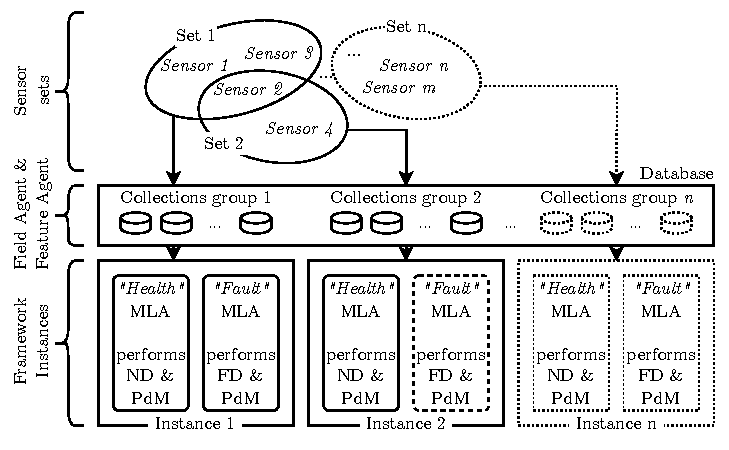
\includegraphics[width=\linewidth]{images/FrameworkInstances.pdf}
    \caption{Multiple instances implementation of the framework. Every instance is linked to a different set of sensors, to monitor different parts of the system.}
    \label{fig:multiple_instances}
\end{figure}


\subsection{Unsupervised Machine Learning Models}

The UML implemented in the framework are: \emph{K-means}, \emph{DBSCAN}, \emph{Gaussian Mixture Model} (GMM), \emph{Isolation Forest} (IF), \emph{Local Outlier Factor} (LOF), \emph{One-Class Support Vector Machine} ($\nu$-SVM).

K-means and DBSCAN are traditionally clustering algorithms, so a custom NM has been developed for these algorithms. For example, if K-means is used, the NM is defined as the distance of a sample from the closest centroid, normalized by the cluster radius. The other models are already commonly used for ND, so the NM has been linked to the \quoted{score} provided by the library functions.

If the UML is trained with faulty data, instead of normal ones, then it performs FD. The NM measures \quoted{how not faulty} the new data are. In this case, the value is transformed into a Fault Metric (FM) with the function $\text{FM} = - \ln(\text{NM} + 1)$ to preserve the coherence (the lower the metric, the healthier the system). 
\section{VALIDATION}
\label{sec:validation}

\subsection{On bearings vibration datasets}

The PC implementation of the framework has been thoroughly tested on a publicly available dataset provided by the Center for Intelligent Maintenance Systems (IMS).
%\footnote{\url{https://www.nasa.gov/intelligent-systems-division/discovery-and-systems-health/pcoe/pcoe-data-set-repository/}}
The dataset contains time series of the vibration of four bearings, for a total of three separate \quoted{run to failure} experiences. The dataset provides information about the location and type of defects observed after each test.

\begin{figure}
    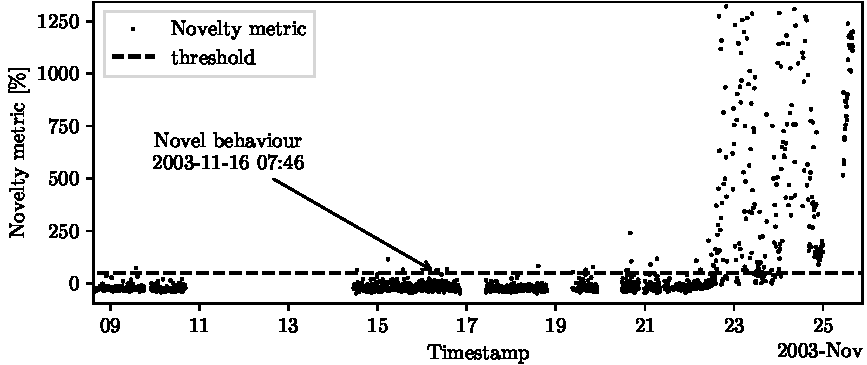
\includegraphics[width=\linewidth]{images/ND_IMS.pdf}
    \caption{Results of ND on the IMS dataset. When the Novelty Metric crosses the threshold, a warning is issued. The malfunction happens at the end of the dataset.}
    \label{fig:ND_IMS}
\end{figure}
\begin{table}
    \centering
    \caption{Comparison of the results for the test n$^\circ$1 of IMS dataset.}
    \label{tab:ims01_comparision}
    \begin{tabular}{lcrr} 
    \toprule
    \textbf{Algorithm} & \textbf{ND event} & \textbf{LT }{[}min] & \textbf{LT }{[}days] \\ 
    \hline
    K-means & 2003-11-16 07:46 & \textbf{13913} & \textbf{9.6} \\
    DBSCAN & 2003-11-22 15:06 & 4833 & 3.3\\
    GMM & 2003-11-22 03:47 & 5513 & 3.8\\
    BGMM & 2003-11-22 03:45 & 5514 & 3.8\\
    $\nu$-SVM & 2003-11-22 14:56 & 4844 &3.3\\
    IF & 2003-11-16 10:08 & 13771 & 9.6\\
    LOF & 2003-11-16 07:48 & 13912 & 9.6\\
    {P2P} without any ML & 2003-11-22 16:06 & 4774 & 3.3\\
    \bottomrule
    \end{tabular}
\end{table}
The ND capability of the framework has been tested using all the UML models. The lead time (LT) elapsed between the ND event and the actual fault is used to compare the models. The results are compared in table~\ref{tab:ims01_comparision}. The evolution of the NM, using a K-means model on a signal of the test N$^\circ$1, is shown in Fig.~\ref{fig:ND_IMS}.

\begin{figure}
    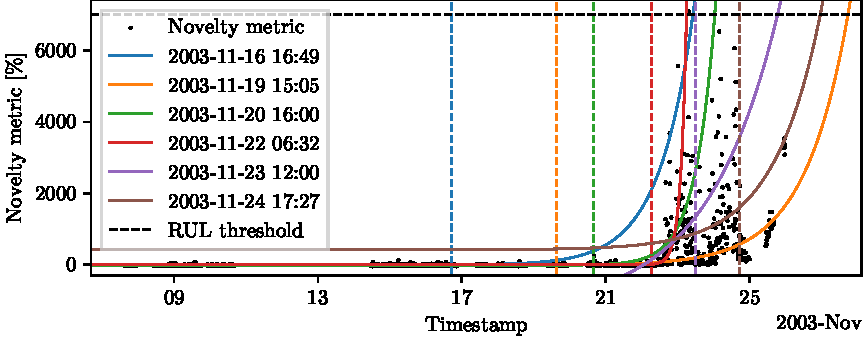
\includegraphics[width=\linewidth]{images/RUL_IMS.pdf}
    \caption{Results of Remaining Useful Life predictions on the IMS dataset. The Vertical lines indicate the time when the predictions are performed. The RUL is the time remaining before the instant when the fitted curve crosses the threshold.}
    \label{fig:RUL_IMS}
\end{figure}
To perform PM, the framework has to estimate the Remaining Useful Life (RUL) of the system. The RUL is predicted computing when a fitted curve crosses a certain threshold. The type of curve to fit is configurable, in this work $y = a \cdot e^{b \cdot x} + c$ has been used. The results of the RUL predictions are shown in Fig.~\ref{fig:RUL_IMS}.

\begin{figure}
    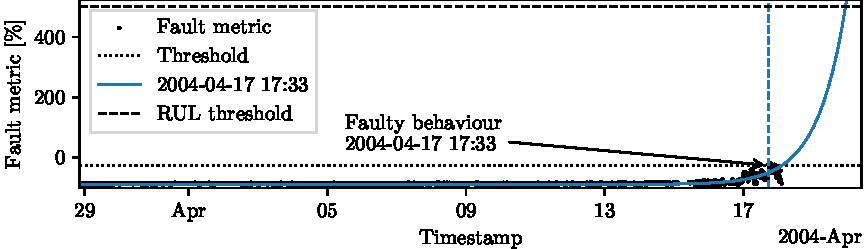
\includegraphics[width=\linewidth]{images/FD_IMS.pdf}
    \caption{Results of FD on the IMS dataset. The malfunction is detected when the Fault Metric crosses the threshold. The RUL is the time remaining before the instant when the fitted curve crosses the threshold.}
    \label{fig:FD_IMS}
\end{figure}
Since the second and third tests of the IMS dataset share the same kind of fault, the framework has been trained to perform FD with the faulty data of the second test and then evaluated on the third. Analogously to the ND, after the FM crosses a certain threshold, a warning is issued and RUL predictions are performed. The results of the FD are shown in Fig.~\ref{fig:FD_IMS}.

\subsection{Laboratory tests}

\begin{figure}
    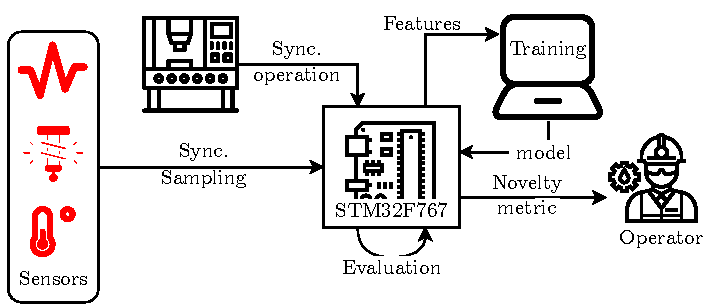
\includegraphics[width=\linewidth]{images/EmbeddedStructure.pdf}
    \caption{Structure of the Edge implementation}
    \label{fig:embedded}
\end{figure}

Since the validation on the IMS dataset has shown that the K-means model is both the simplest and the most effective, it has been deployed on the Edge implementation. In the first phase, the framework gathers the data, extracts the features and sends them to a PC. The UML model is trained on the PC and then sent back to the Edge. After, the microcontroller autonomously evaluates the status of the maintained system. The structure of the Edge implementation is shown in Fig.~\ref{fig:embedded}.

\begin{figure}
    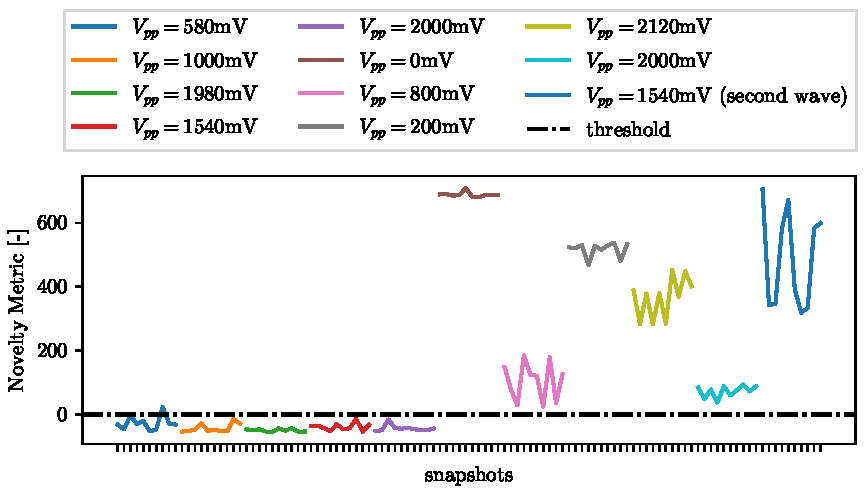
\includegraphics[width=\linewidth]{images/Test02_LOF.pdf}
    \caption{Results of laboratory test on the shaker. The first five lines are evaluations of known vibrations, correctly evaluated as normal samples. The remaining lines are the successful detections of the novelty of new vibrations.}
    \label{fig:shaker}
\end{figure}

Extensive tests have been performed on a laboratory shaker, simulating the vibrations generated by a generic mechanical system. The tests have been carried out to evaluate the sensitivity to variations in both amplitude and frequency content of the vibrations. In Fig.~\ref{fig:shaker} the results of the ND are shown. The first five lines are novelty evaluations a repetition of the same signals used for training, and the remaining lines are the successful detections of the novelty.

A second series of tests has been performed mounting the accelerometer on a linear actuator. The axis of the accelerometer has been aligned with the direction of the movement of the actuator, to sense more the acceleration actuated rather than the vibrations. A set of predefined movement profiles has been used for training, while another set for testing. This series of tests exploited a high number of non-significant features. This is because the WPD gave high resolution on a wide range of frequency content, but the actuator excited only a few, and very low, frequencies. The remaining features were almost all noise, and the standardization procedure had the side effect of amplifying them to the same level as the significant ones. An effort has been made to fine-tune the model to reduce the impact of the noise (see Fig.~\ref{fig:linear}, models 1 to 4). The best result, however, has been obtained by removing the less informative features and using a reduced feature space. The benefit of this approach is evident in Fig.~\ref{fig:linear}, as \quoted{Model 5} shows a clear and sharp detection of the alternating pattern between known and unknown movement profiles.


\begin{figure}
    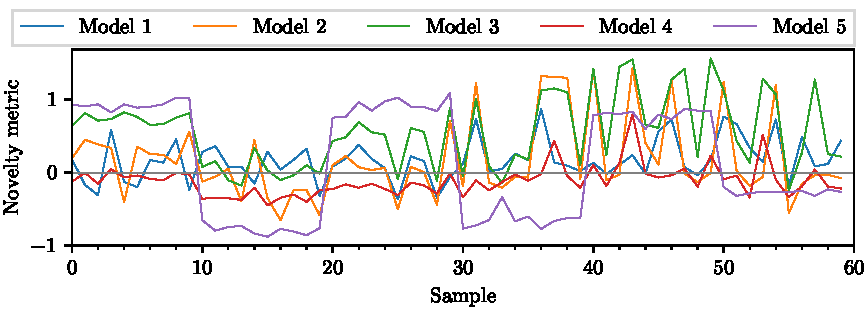
\includegraphics[width=\linewidth]{images/linear.pdf}
    \caption{Results of laboratory test on linear actuator acceleration profiles}
    \label{fig:linear}
\end{figure}
\section{CONCLUSION AND FUTURE WORK}


\end{document}
